%!TEX root = ../main.tex
The requirements state that it should be simple to add additional sensors to the system.
Adding a sensor includes creating a way of easily accessing and showing the data on the observing system.
This section will explain the design of the backend that will provide this functionality.
\martin{Is any of this backend?}

\subsection{Data Format}
Depending on where the data comes from it may be inherently different. 
The interpretation of data is therefore not uniform across the entire system.
For this reason, it is necessary to create a system that is agnostic with respect to the type and amount of data being handled.
In section \ref{sub:CAN_protocol} a description of the node and message identification system is given.
The node ID and message type identifiers are decided by the implementer and together they provide a unique, 11 bit identifier, the message ID, for the type of data in the message.
Since the message ID is capable of uniquely identifying the data, it will be used in storing the data.
Additionally each message will be associated with a 4 byte timestamp.
This timestamp is given as the time in milliseconds since synchronization and is associated with message type 1.

\subsection{Front End Architecture}\label{sec:frontend}
An overview of the functionality can be seen in figure \ref{fig:backendconcept}.
As can be seen, this architecture provides the link between the receiving program (socat) and a potential \acs{gui}.
Upon receiving a message from the go-kart, socat will pipe the raw message to the interpreter.
The interpreter will proceed to extract the message ID, the timestamp and the data.
These are then put into a fifo buffer which will contain the latest 1024 data points for a given message ID.
\martin{does that mean that there are upwards of 1000 independent fifos? Looking at figure~\ref{fig:backendconcept}, it seems like is a three part FIFO, where messages get mixed between each other}
\thomas{Make the figure more clear.}
One of the requirements of this system is that it should be easily expandable.
A consequence of this is that adding a new node on the system should require as few changes to the code as possible.
Making this backend agnostic with respect to the type of data means that no changes are required when adding different nodes with different data types.
However, full agnosticity throughout the entire backend would mean that the GUI programmer needs to know how to handle the binary data.
Instead, it was decided to let the backend consist of a number of functions, written specifically for each node.
The GPS node, for instance, may have a \texttt{get\_latitude()} function.
In this manner, an API can be created which provides the GUI with access to the parameters that needs to be shown.
The complete code can be found on the associated github repository in \path{code/backend/}.
As a note, throughout this section it is assumed that the messages are of string type.
Clearly, this is hugely inefficient as these are string representations of binary numbers.
In testing the software this approach simplified the process greatly and was due to time pressure.
It is unlikely that this choice will pose any issues in terms of performance since this code will be running on a PC, a platform that is several orders of magnitude faster than the ZB.

\begin{figure}
	\includegraphics[width=\linewidth]{graphics/backend_concept}
	\caption[Overview of the backend functionality.]{Overview of the backend functionality. 
	Messages are received over wifi from the go-kart. 
	An interpreter reads the message to determine the MessageID (MSGID), timestamp (T) and the data. 
	All information is made available to a \acs{gui} through the backend.}
	\label{fig:backendconcept}
\end{figure}

\begin{figure}[H]
	%\missingfigure{Backend Class Diagram}
	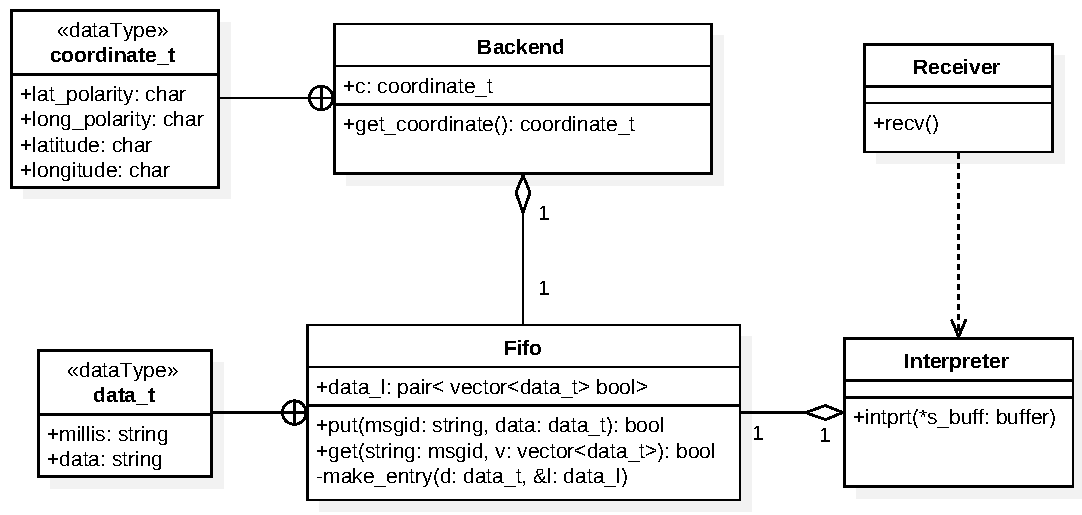
\includegraphics[width=\linewidth]{graphics/backend_class_diagram}
	\caption[Backend class diagram.]{Classdiagram of the backend.}
	\label{fig:backendclass}
\end{figure}
\thomas{Changes to figure \ref{fig:backendclass}: all class names with small letters, backend should be called frontend, also figure~\ref{fig:backendconcept}}
From figure~\ref{fig:backendconcept}, a class diagram has been created.
This can be seen on figure \ref{fig:backendclass}.
The functionality is implemented in four classes, each of which will be explained in more detail below.

\subsubsection*{\texttt{receiver} class}
This class is run in a separate thread.
It continuously listens to std::io, waiting for input from the go-kart.
Upon receiving a message, it is put into a message buffer maintained by interpreter.

\subsubsection*{\texttt{interpreter} class}\label{sub:backend_intepreter}
As mentioned, this class holds a message buffer, it is shown in code \ref{code:msgbuffer}.
The buffer can be accessed from the receiver thread indirectly by a call to \texttt{put()} and the interpreter thread continously checks if data is present in the buffer.
Since these threads are run simultaneously it is necessary to use a mutex to avoid race conditions.
Whenever a message is put in the buffer, it is split into its three components, a 10 bit message id, a 4 byte timestamp and a string of data of arbitrary length.
On figure \ref{fig:backendmsg} is a depiction of the messagetype.
\begin{figure}[H]
	%\missingfigure{Backend Message (msgid/timestamp/data)}
	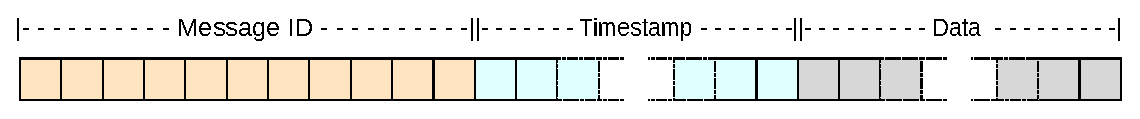
\includegraphics[width=\linewidth]{graphics/backend_message}
	\caption[Front end message.]{Depiction of the message sent over wifi. The message id is the same 11 bit identifier used in the CAN network.
	The timestamp is a 4 byte value containing the number of milliseconds since synchronization.
	The data field can be of arbitrary length.}
	\label{fig:backendmsg}
\end{figure}

Once split, the information is stored using from the \texttt{fifo::put()}. 
\begin{lstlisting}[caption=Buffer for holding incoming messages.,label=code:msgbuffer]
struct buffer 
{
  std::vector<std::string> strings;
  std::mutex mutex;
};
\end{lstlisting}
\subsubsection*{\texttt{fifo} class}
This class implements a hashmap and functions to insert and extract data from the map.
Each messageid has a flag associated with it to signal whenever new data is available.
The hashmap uses the message id as the key and the data is \texttt{std::pair<std::vector<data\_t>, bool>}.
That is, each message id is associated with a list of \texttt{data\_t} and a \texttt{bool} used as a flag.
As with the buffer in the interpreter class, the fifo will be accessed from two threads running simultaneously and as such, mutexing is necessary.
Mutexing is done on the \texttt{put()} and \texttt{get()} functions directly.
The \texttt{put()} function is shown in code \ref{code:fifoput}.
It takes a message id and a data frame as arguments.
The \texttt{data\_t} type is a struct containing a timestamp and a string of data.
Initially it will attempt to lock the mutex, if it fails, the function returns false and the caller will have to try again until successful.
When the mutex is locked, it searches through the hashmap for the message id.
If the search fails, this is the first message from that node, with that message type and a new entry is made in the hashmap.
If the search succeeds the new data point is pushed onto the end of the data list.
If there are 1024 points in the list already, the first element is deleted.
Before returning true to indicate that the data has been put into the fifo, the flag is set high and the mutex is unlocked.

\begin{lstlisting}[caption=Function used to insert new data into the hashmap.,label=code:fifoput]
bool fifo::put(std::string msgid, data_t data)
{
	if(mutex.try_lock())
	{	
		if (buffer.find(msgid) == buffer.end())
		{
			data_l list;
			make_entry(data,list);

			buffer.emplace(msgid,list);
		}
		else
		{
			buffer[msgid].first.push_back(data);
			
			if(buffer[msgid].first.size() > 1023)
			{
				buffer[msgid].first.erase(buffer[msgid].first.begin());
			}
		}
		sem_set(msgid);
		mutex.unlock();
		return true;
	}
	return false;
}
\end{lstlisting}

\texttt{get()} works similarly by first locking the mutex and then checking for the existence of the message id.
If the message id is present, the flag is cleared, the data list is copied to the address given in the function call and true is returned to indicate success.

\subsubsection*{\texttt{frontend} class}
As mentioned previously, the backend is a collection of functions which interpret and present the data collected in the fifo for use in a potential GUI.
This aims to hide some of the complexity of the underlying system from the GUI programmer.
Any number of functions can be added to this class depending on the needs of the sensor.
The general structure of a function can be seen in code \ref{code:frontendfunction}.

\begin{lstlisting}[caption=Function template for accesing data in fifo.,label=code:frontendfunction]
<PARAMETER_TYPE> frontend::get_<PARAMETER>()
{
	std::vector<data_t> v;

	while(!fifo_o->get(<MESSAGE_ID>, v));

	if (!v.empty())
	{
		double t = std::stoi(v.back().millis);
		std::string d = v.back().data;

		/*Decipher d*/
	}

	return <PARAMETER_TYPE>;
}
\end{lstlisting}